\chapter{Introducci�n}

Debido a la creciente disponibilidad de las plataformas m�viles y el gran poder de procesamiento con el que cuentan, el n�mero de aplicaciones m�viles ha crecido de manera significativa. Dichas plataformas cuentan con sistemas de adquisici�n de audio, video y una variedad de sensores como por ejemplo aceler�metro y giroscopio, lo que las transforma en sistemas ideales para desarrollar aplicaciones de procesamiento multimedia.\\

Adem�s de desarrollar sobre plataformas m�viles, este proyecto busca contribuir al desarrollo de software que fomente contenidos educativos y art�sticos, generando as� un espacio que pone la tecnolog�a al servicio de la cultura y la sociedad. As� entonces sigue la l�nea de generar formas innovadoras de presentar contenidos por parte de museos y galer�as de arte de manera de ser part�cipe activo en propuestas que estimulen el acercamiento de j�venes y adultos a descubrir una manera distinta de vivir el arte.\\

Ya hace algunos a\~nos que varios museos de distintas partes del mundo han comenzado a ver la \textit{realidad aumentada} como una alternativa muy interesante para agregar un atractivo m�s dentro del arte. Sin embargo, si bien han comenzado a aparecer cada vez m�s aplicaciones interactivas para museos, esta es un �rea muy reciente y en la que todav�a queda un camino muy largo por recorrer.\\

Es posible definir la realidad aumentada (AR del ingl�s \textit{Augmented Reality}) como una vista directa o indirecta en tiempo real, de alg�n elemento o escena f�sica del mundo real, a la que se le agrega informaci�n de manera virtual o digital mediante el uso de herramientas computacionales \cite{furht11}. Cuando se genera una escena por medio de la realidad aumentada, conviven en ella elementos reales con elementos virtuales que buscan verse tan reales como se pueda. Es basicamente un juego de percepciones.\\
La realidad aumentada es un �rea que se encuentra en pleno desarrollo y todo el tiempo aparecen ideas novedosas y muy interesantes, lo que la hace por dem�s apasionante. En la Figura \ref{fig: arIntro} se puede ver un ejemplo que resume varias caracter�sticas que representan este concepto y que durante el presente proyecto ser�n detalladas.

\begin{figure}[h!]
\centering
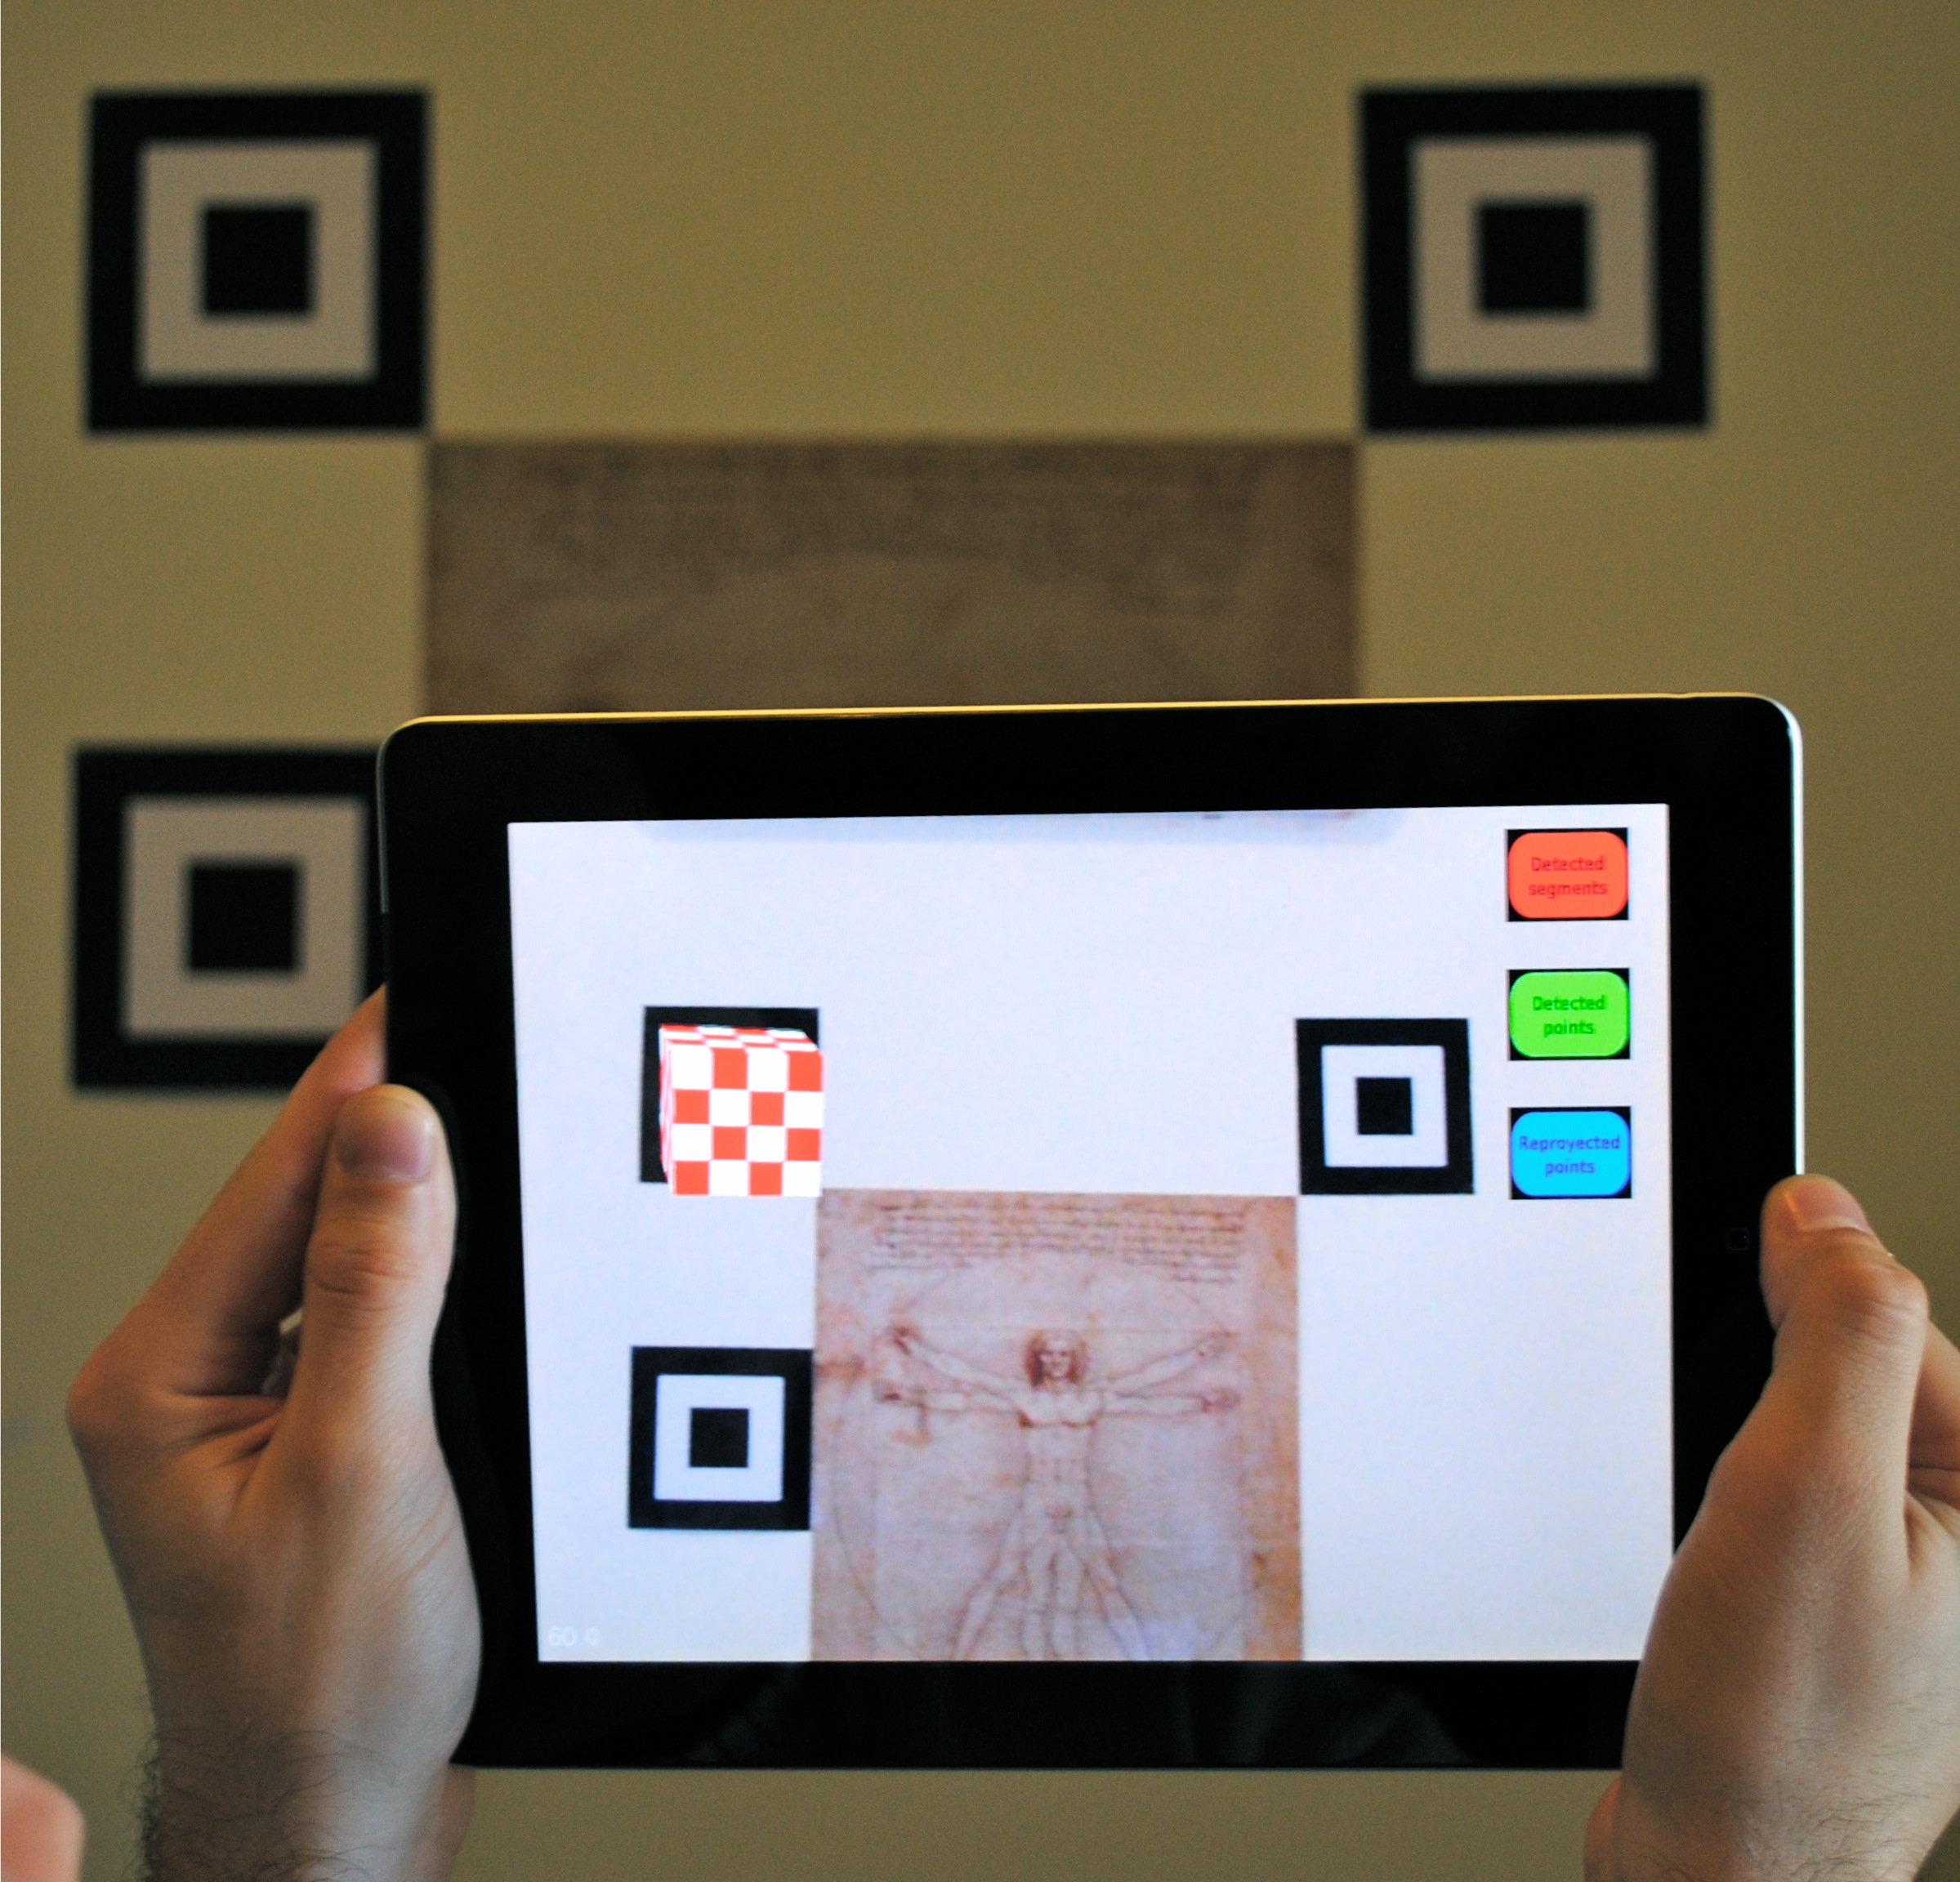
\includegraphics[scale=0.15]{figs_intro/arIntro.png}
\caption{Ejemplo de realidad aumentada}
\label{fig: arIntro}
\end{figure}


